%!TEX root = paper.tex

\newcommand{\foveatedExampleFigure}{

\begin{figure}[h]
  \centering
    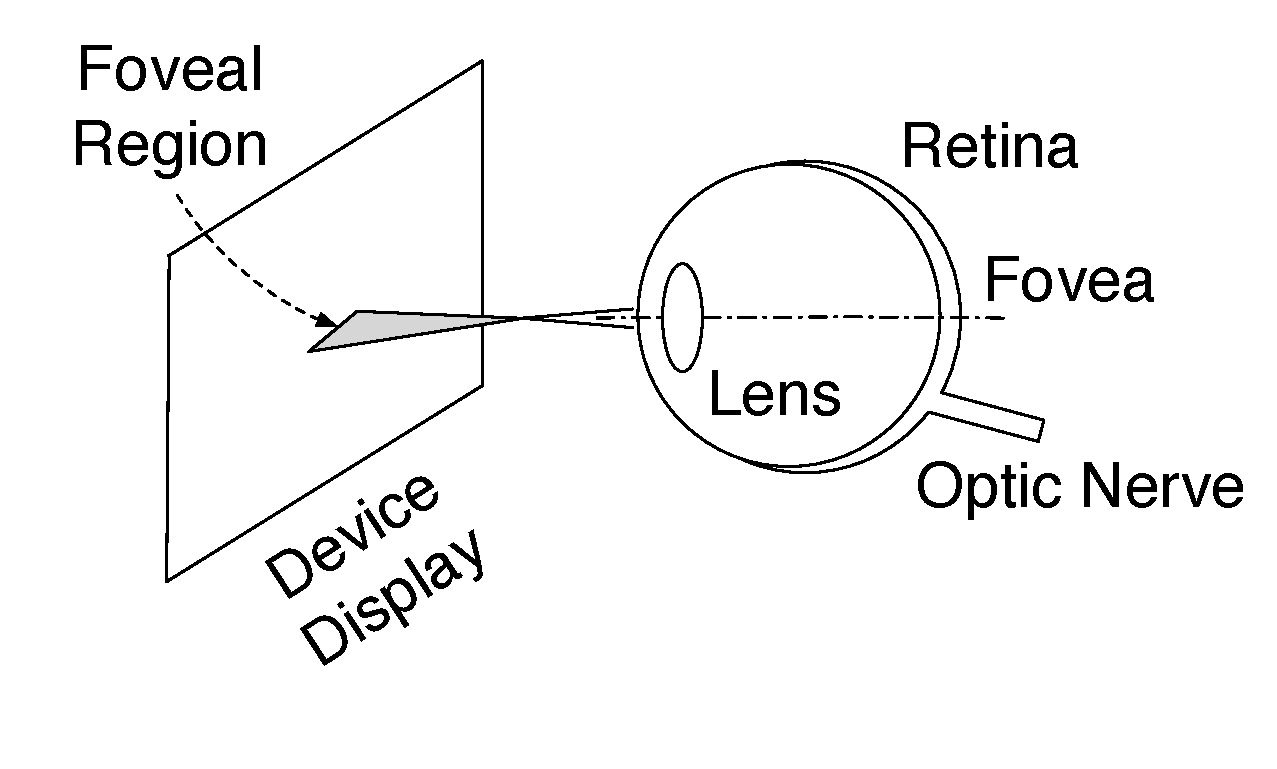
\includegraphics[width=\linewidth]{tvarch-figs/foveated-eye.pdf}
    \caption{The human eye only perceives the foveal region at full resolution~\cite{foveated-coding}.}
    \label{subfig:eye}
    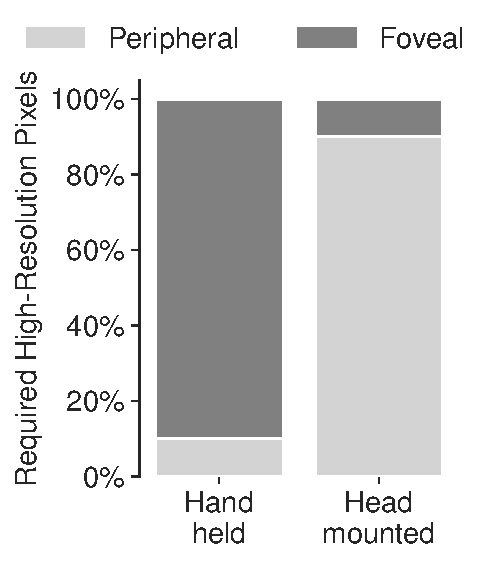
\includegraphics[width=\linewidth]{tvarch-figs/peripheral-pixels.pdf}
    \caption{Foveal region of display devices~\cite{patney2017perceptual}.}
    \label{subfig:breakdown}
  \caption{When viewing a VR display at close distance, only a small fraction of pixels ($<10\%$) are foveal and viewed at high resolution. VR video compression exploits this feature with \emph{foveated compression}.}
  \label{fig:foveal-motivation}
\end{figure}
}

\newcommand{\vdecBaselineArchFigure}{
\begin{figure}[h]
  \centering
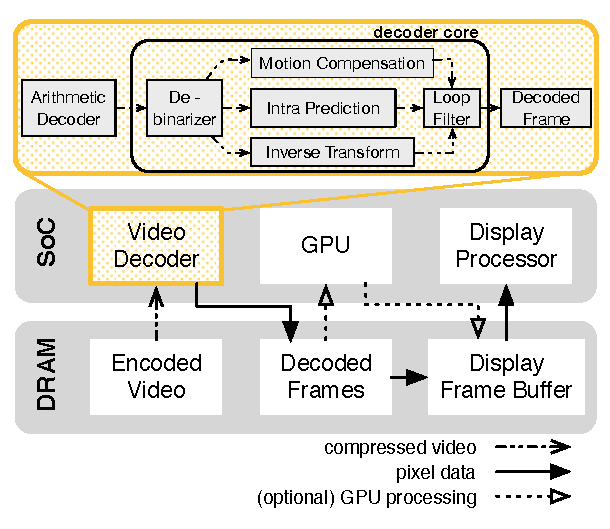
\includegraphics[width=\linewidth]{tvarch-figs/system-arch.pdf}
\caption{System architecture of typical video playback flow on mobile/VR SoC.}
\label{fig:vdec-arch}
\end{figure}
}

\newcommand{\vdecCTUTimingFigure}{

\begin{figure*}[h]
    \centering
    \begin{minipage}[b]{.375\textwidth}
        \centering
        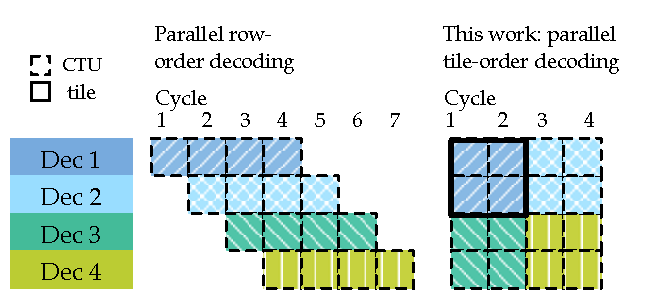
\includegraphics[width=\linewidth]{tvarch-figs/decode-ctu-timing.pdf}
        \caption{Decoding \emph{tiles} in parallel, rather than \emph{rows}, removes row-dependencies.}
        \label{fig:ctu-timing}
    \end{minipage} \hfill
    \begin{minipage}[b]{0.6\textwidth}
        \centering
        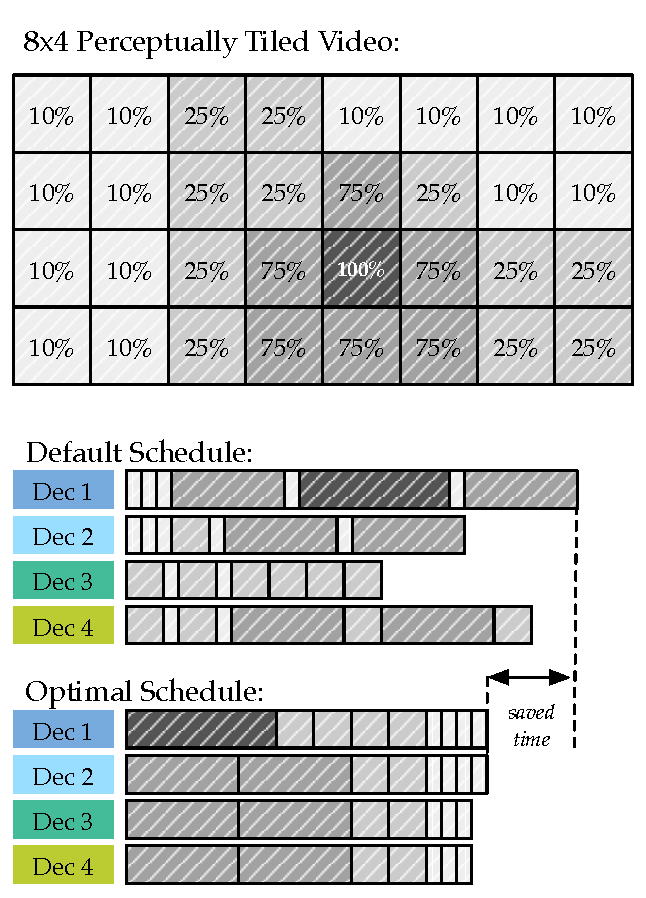
\includegraphics[width=\linewidth]{tvarch-figs/optimal-scheduling.pdf}
        \caption{Optimal scheduler for tiled video with heterogeneous bitrates.}
        \label{fig:tile-schedule}
    \end{minipage}
\end{figure*}
}



\newcommand{\vdoOverview}{
\begin{figure*}[h]
  \centering
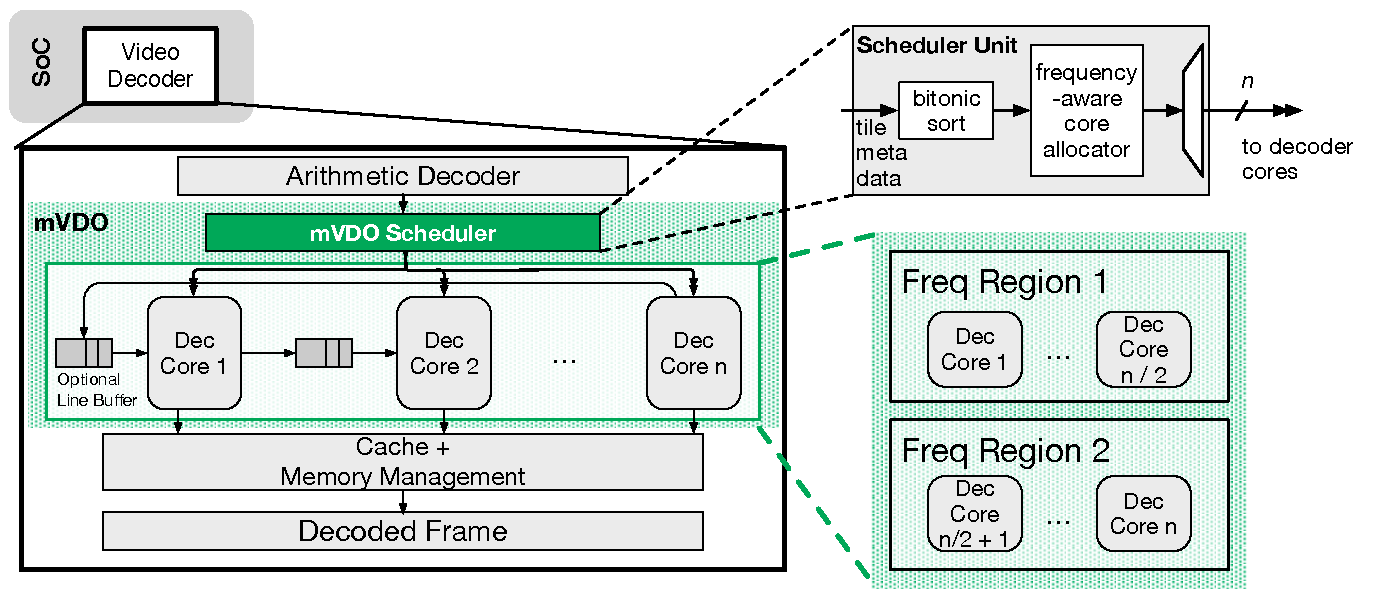
\includegraphics[width=.7\linewidth]{tvarch-figs/mvdo-extended.pdf}
\caption{\nameArch accelerator with heterogeneous parallel decoder cores. \nameArch uses a custom scheduler optimized for processing tiled VR video to efficiently distribute work to decode cores. \nameArch maps video tiles to decode cores in different frequency regions to further improve energy consumption, allocating tiles based on the complexity of the video tile.}
\label{fig:mvdo-arch}
\end{figure*}
}

\newcommand{\vdoprofOverview}{
\begin{figure}[h]
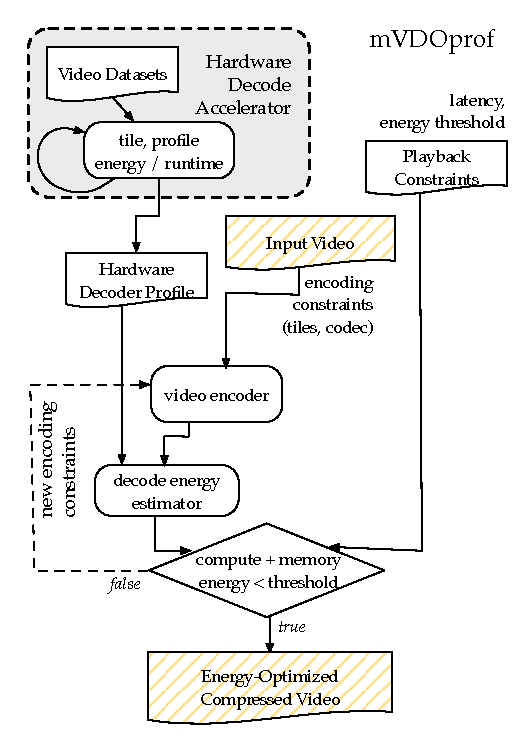
\includegraphics[width=.9\linewidth]{tvarch-figs/vdoprof2.pdf}
\caption{The \nameArchprof framework flow helps VR developers optimize energy consumption of their videos for hardware decoders. \nameArchprof generates energy profiles for video decode architectures and suggests energy-optimal tile configurations for playback constraints.}
\label{fig:vdo-prof}
\end{figure}
}

\newcommand{\perceptualCompressionEnergyFigure}{
  \begin{figure}[h]
    \centering
      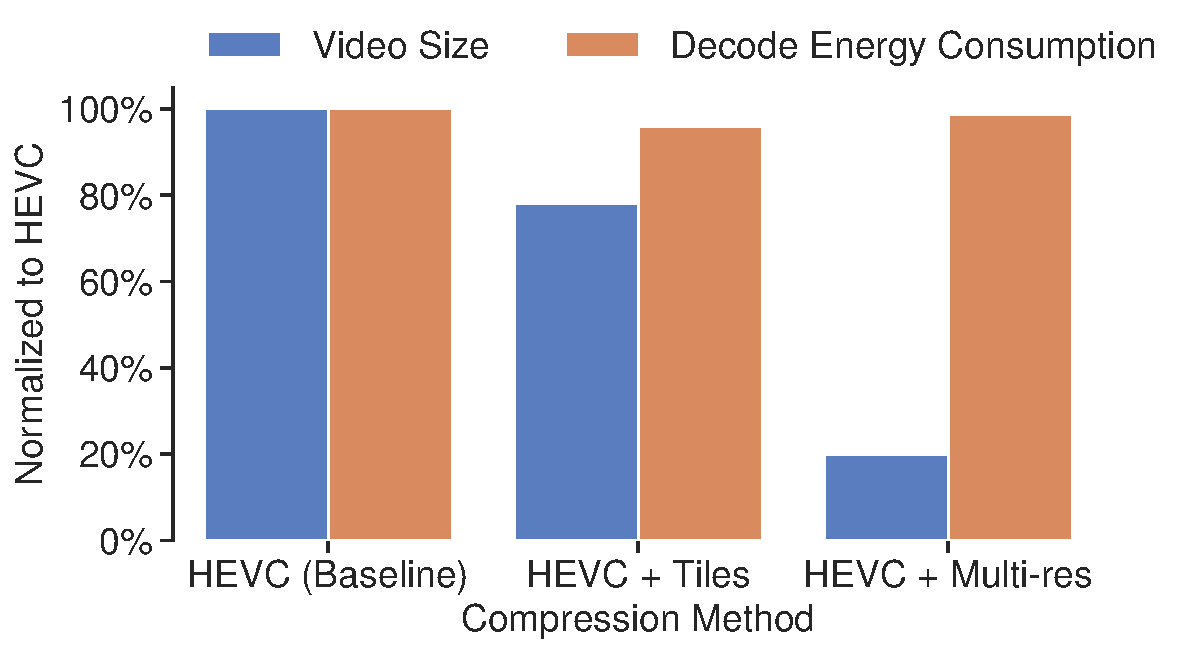
\includegraphics[width=\linewidth]{tvarch-figs/perceptual-energy-opportunity.pdf}
      \caption{Normalized video size and decode energy consumption on mobile SoC.}
      \label{fig:mem-compute}
      \end{figure}%
}
\newcommand{\coresVsDecodeSpeedupFigure}{
  \begin{figure}[h]
    \centering
      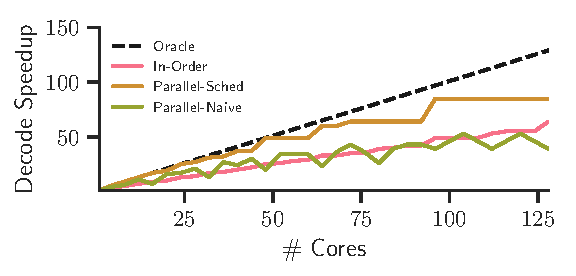
\includegraphics[width=\linewidth]{tvarch-figs/cores-v-decode-speedup.pdf}
      \caption{Decode performance for in-order and \nameArch's parallel decoding, with and without optimal scheduling.}
      \label{fig:cores-decode}
      \end{figure}%
}

\newcommand{\coresVsEnergySpeedup}{
\begin{figure}[h]
  \centering
    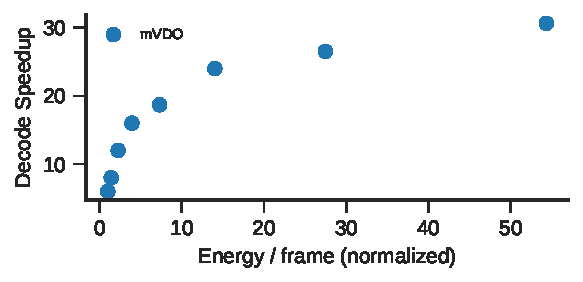
\includegraphics[width=\linewidth]{tvarch-figs/cores-v-power-area-speedup.pdf}
    \caption{Tradeoff between energy consumption per frame and decode speedup as more cores are added to \nameArch. This figure references a homogenous-core design. \todo{still need DVFS results} }
    \label{fig:energy-speedup-cores}
    \end{figure}%
}

\newcommand{\motivationComputeMemEnergyTime}{

\begin{figure*}[h]
    \centering
    \begin{minipage}[h]{.48\textwidth}
        \centering
        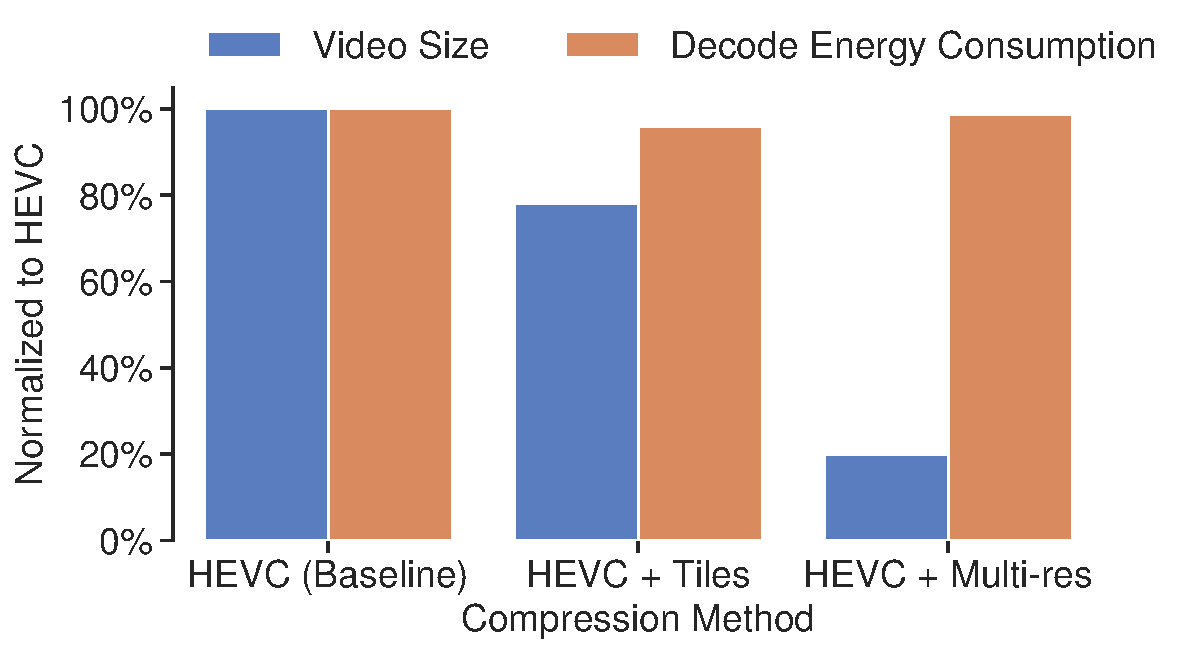
\includegraphics[width=.95\linewidth]{tvarch-figs/perceptual-energy-opportunity.pdf}
        \caption{Memory energy consumption decreases by using perceptual compression, but decoders do not take advantage of this.}
        \label{fig:mot-percept-energy}
    \end{minipage} \hfill
    \begin{minipage}[h]{0.48\textwidth}
        \centering
            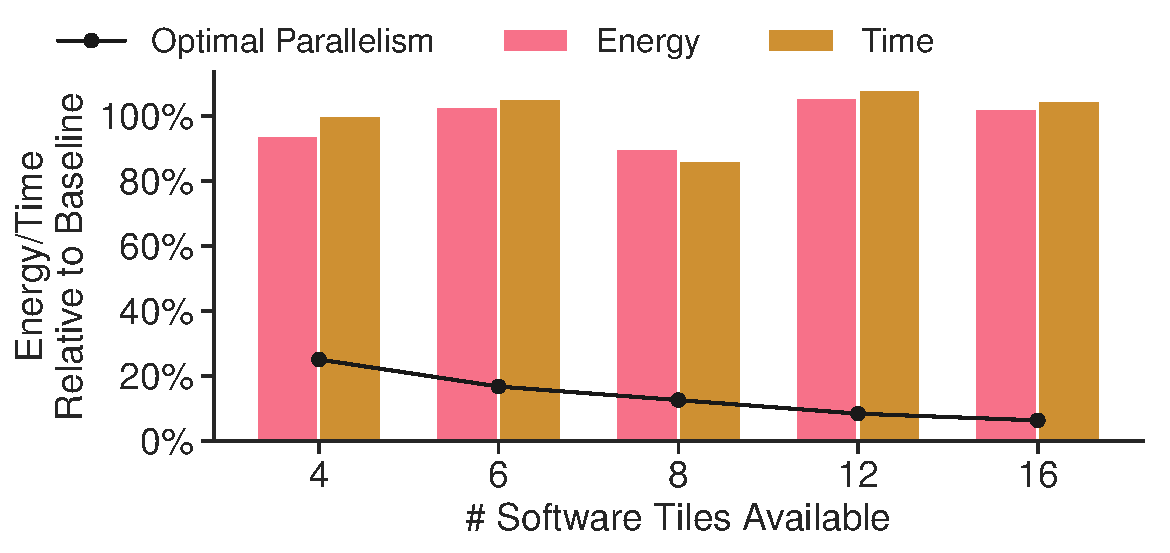
\includegraphics[width=\linewidth]{tvarch-figs/motivation-single-tile-energy-time.pdf}
            \caption{VR video hardware decoders do not take advantage of video tile parallelism. Even as more parallelism is made available, decode energy and runtime remain approximately stagnant.}
        \label{fig:mot-tile-energy-time}
    \end{minipage}
\end{figure*}

}


\newcommand{\perceptualCompressionExampleFigure}{


\begin{figure}
        \centering
        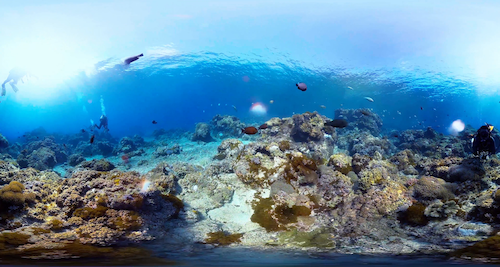
\includegraphics[width=\linewidth]{tvarch-figs/perceptualCompressionExample/diving.png}
        \caption{Input 4K video frame from VR-360 dataset~\cite{vr360-mmsys17}. Original size is 19 MB.}
        \label{subfig:og-stil}
      \quad
        \centering
        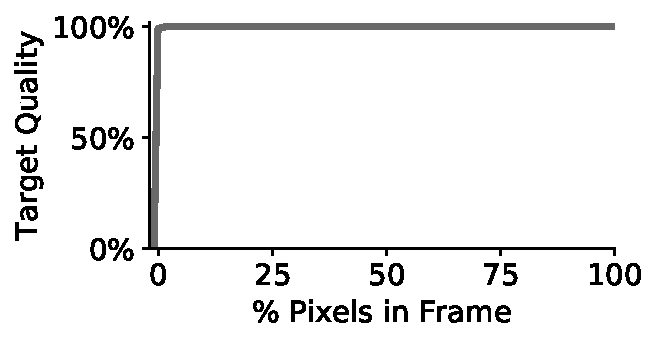
\includegraphics[width=\linewidth]{tvarch-figs/cdf-baseline.pdf}
        \caption{CDF of quality target for pixels in frame.}
        \label{subfig:og-cdf}

      \centering
      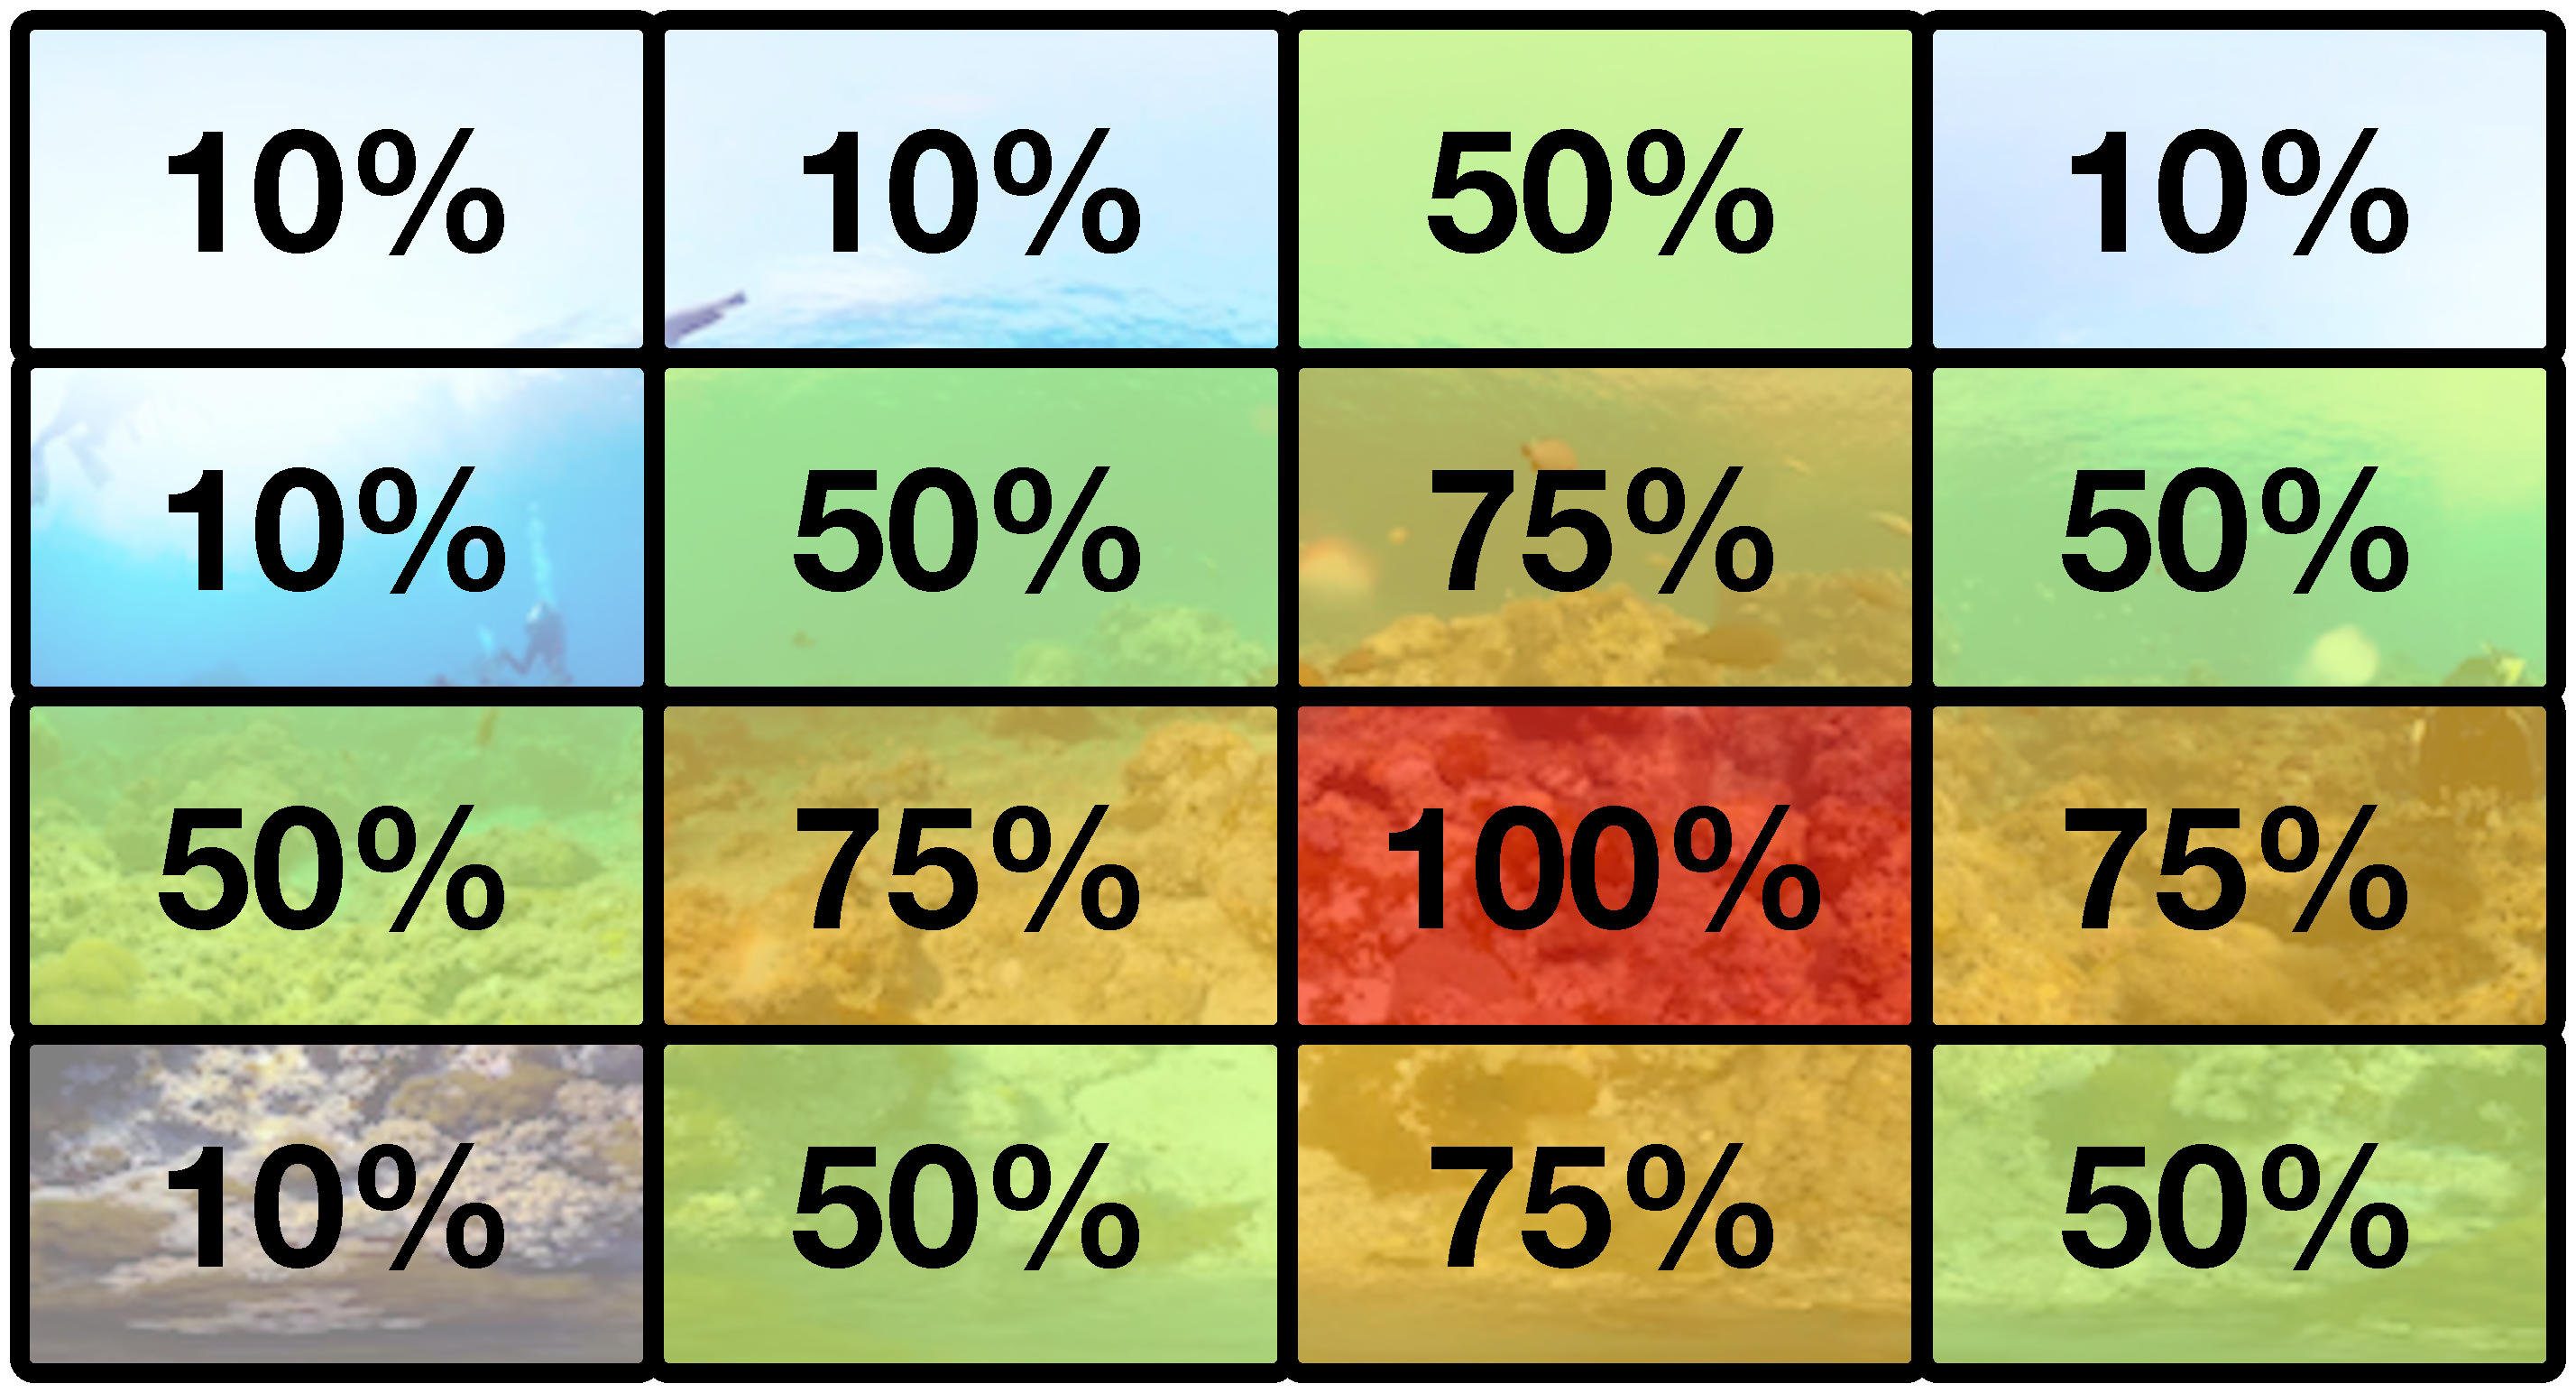
\includegraphics[width=\linewidth]{tvarch-figs/perceptualCompressionExample/tiled-example.pdf}
      \caption{Tiled compression, centered around the fovea. Video size is 11 MB.}
      \label{subfig:tiled-still}
      \quad
        \centering
        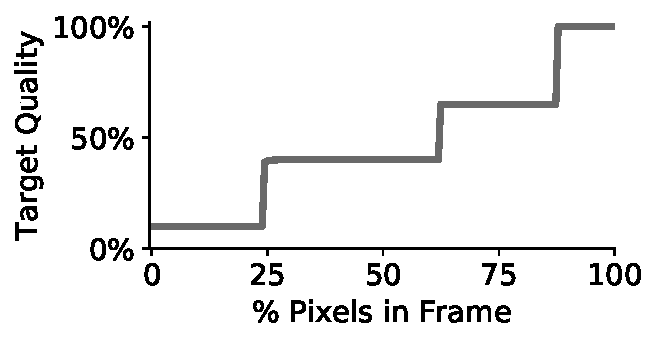
\includegraphics[width=\linewidth]{tvarch-figs/cdf-tiled.pdf}
        \caption{CDF of quality target for pixels in frame.}
        \label{subfig:tiled-cdf}

      \centering
      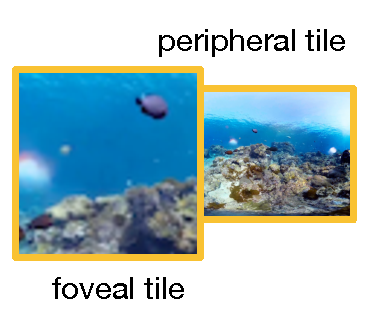
\includegraphics[width=\linewidth]{tvarch-figs/perceptualCompressionExample/multi-scale.pdf}
      \caption{Multi-resolution compression: two tiles for foveal and peripheral areas. Video size 5 MB. }
      \label{subfig:fov-still}
      \quad
        \centering
        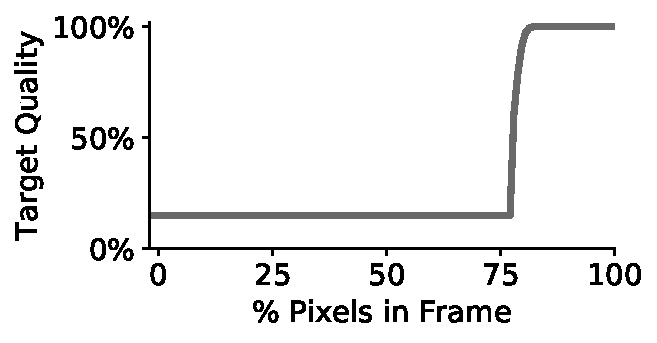
\includegraphics[width=\linewidth]{tvarch-figs/cdf-layered.pdf}
        \caption{CDF of quality target for pixels in frame.}
        \label{subfig:layered-cdf}

    \caption{Example video still and visualizations of tiled and multi-resolution video compression. These VR video compression methods use 40-75\% less storage by distributing quality across video tiles.}
    \label{fig:example-vid-compressed}
\end{figure}

}

\newcommand{\dvfsEnergySpeedup}{
\begin{figure*}[h]
    \centering
      \centering
      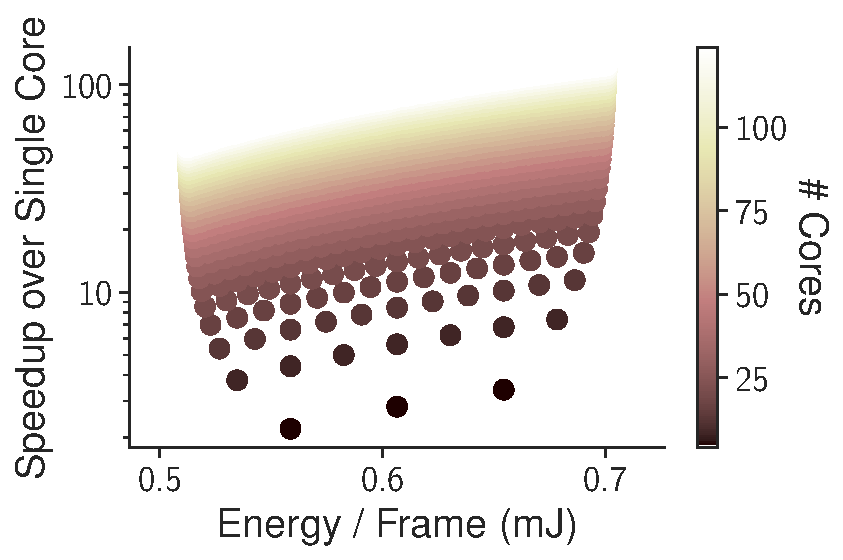
\includegraphics[width=\linewidth]{tvarch-figs/dvfs-energy-speedup-all.pdf}
      \caption{Energy consumption and speedup of \nameArch, over a sweep of 2000 configurations of multi-core, heterogeneous frequency setups. }
      \label{subfig:dvfs-all}
      \quad
        \centering
        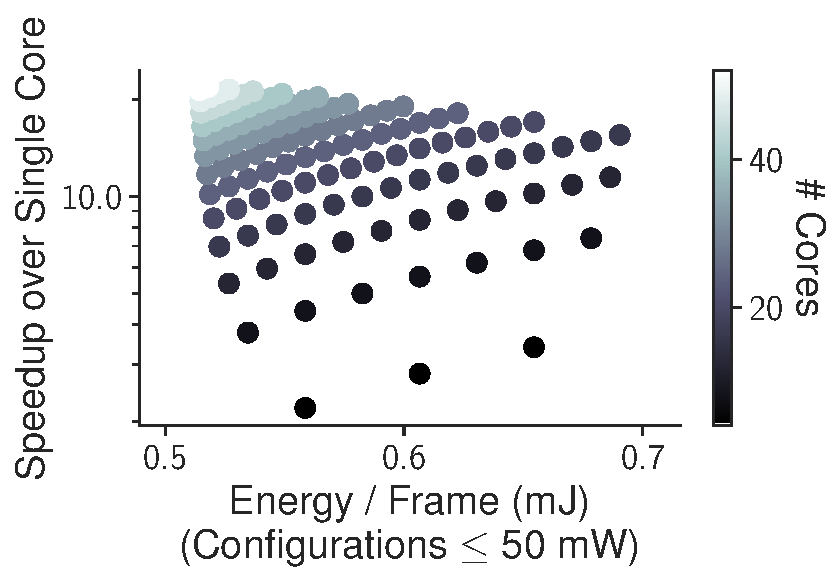
\includegraphics[width=\linewidth]{tvarch-figs/dvfs-energy-speedup-sub50mw.pdf}
        \caption{Energy consumption and speedup of \nameArch, now filtered to only show results under 50 mW.}
        \label{subfig:dvfs-sub50}
      \caption{We swept over heterogeneous parallel configurations for our video decoder, varying the number of cores from 4 - 128 and the number of fast and slow cores for each core count. We find a Pareto-frontier of optimal energy-speedup configurations (a). After filtering based on power consumption (b), the spread of optimal energy-speedup configurations shifts. The best Pareto-optimal point under 50 mW is a 52-core design. }
      \label{fig:dvfs-exploration}
\end{figure*}
}

\newcommand{\evalEnergyPower}{
\begin{figure}[h]
    \centering
          \centering
          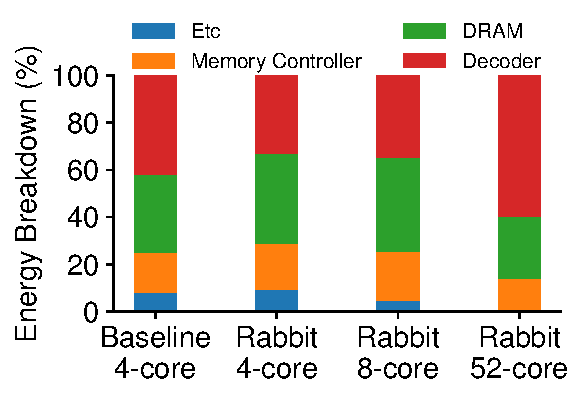
\includegraphics[width=\linewidth]{tvarch-figs/eval-energy-breakdown.pdf}
          \caption{Energy breakdown. }
          \label{subfig:eval-energy-percent}
          \quad
            \centering
            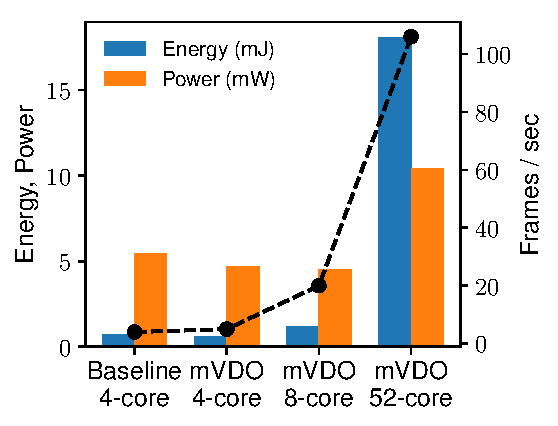
\includegraphics[width=\linewidth]{tvarch-figs/eval-power-energy-total.pdf}
            \caption{Energy consumption and total power consumption.}
            \label{subfig:eval-power-energy}
          \caption{Energy breakdown of \nameArch components; energy and power consumption on a single video. Our 4-, 8-, and 52-core designs improve decode latency by .25 - 25$\times$ while keeping power under 15 mW. }
\end{figure}
}

\newcommand{\evalRegularTileEnergy}{
\begin{figure}[h]
  \centering
    \centering
    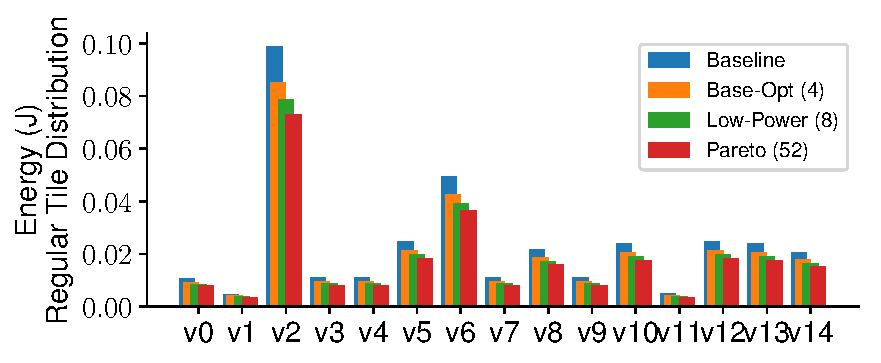
\includegraphics[width=\linewidth]{tvarch-figs/eval-energy-regular-vbench.pdf}
    \caption{\texttt{vbench} energy consumption results for regularly distributed tiles. }
    \label{subfig:eval-energy-regular-vbench}

  \centering
  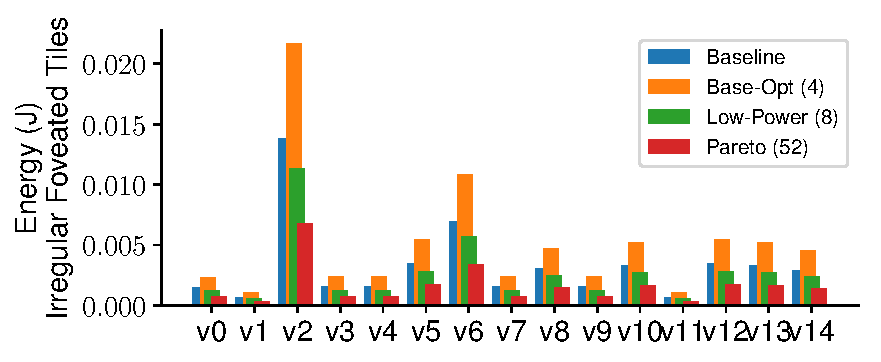
\includegraphics[width=\linewidth]{tvarch-figs/eval-energy-fov-vbench.pdf}
  \caption{\texttt{vbench} energy consumption results for irregular foveated tiles. }
  \label{subfig:eval-energy-fov-vbench}

  \centering
  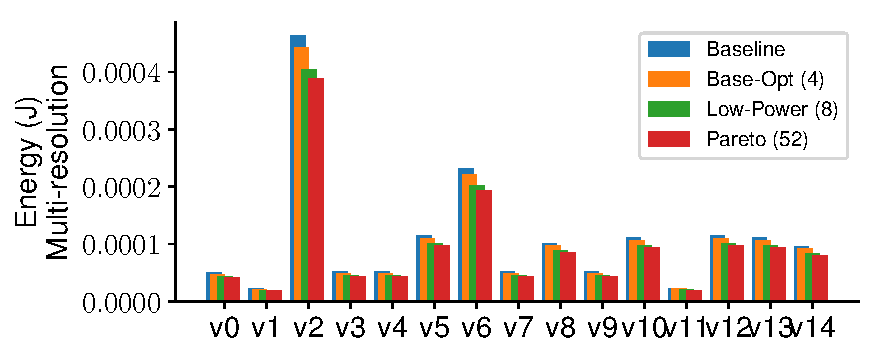
\includegraphics[width=\linewidth]{tvarch-figs/eval-energy-multi-vbench.pdf}
  \caption{\texttt{vbench} energy consumption results for multi-resolution foveation. }
  \label{subfig:eval-energy-multi-vbench}
\caption{Energy consumption for decoding \texttt{vbench} videos. \texttt{vbench} videos range in resolution and show a commensurate range in energy consumption. \nameArch reduces energy consumption for all compression styles but is most scalable for foveated tiles and lowest-energy for multi-resolution foveation.}
\end{figure}

\begin{figure}[h]
  \centering
    \centering
    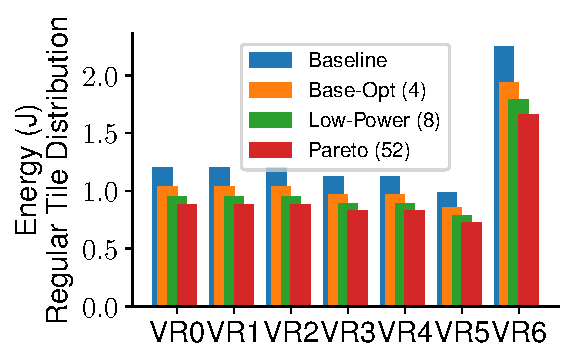
\includegraphics[width=.675\textwidth]{tvarch-figs/eval-energy-regular-vr.pdf}
    \caption{\texttt{vr-360} energy consumption results for regularly distributed tiles.}
    \label{subfig:eval-energy-regular-vr}

  \centering
  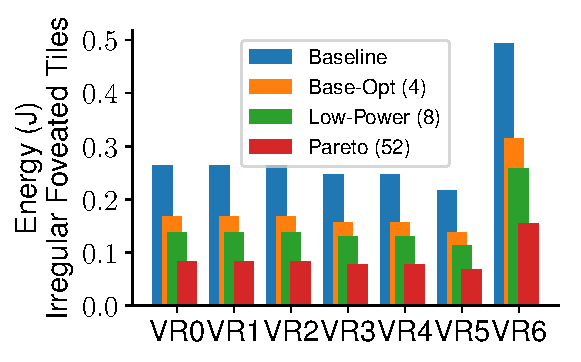
\includegraphics[width=.675\textwidth]{tvarch-figs/eval-energy-fov-vr.pdf}
  \caption{\texttt{vr-360} energy consumption results for irregular foveated tiles.}
  \label{subfig:eval-energy-fov-vr}

  \centering
  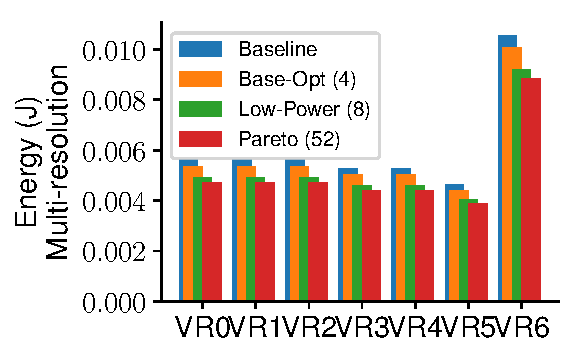
\includegraphics[width=.675\textwidth]{tvarch-figs/eval-energy-multi-vr.pdf}
  \caption{\texttt{vr-360} energy consumption results for multi-resolution foveation.}
  \label{subfig:eval-energy-multi-vr}
\caption{Energy consumption for decoding \texttt{vr-360} videos. \texttt{vr-360} show greater benefit from \nameArch's scalability, indicating that larger, high-resolution VR content benefits more from \nameArch's optimizations.}
\end{figure}
}


\newcommand{\dvfsConfigTable}{
\begin{table}[h]
  \centering
  \caption{\nameArch Evaluation Design Points and Configuration Characteristics}
  \label{tab:dvfs-configs}
  \begin{tabular}{llll} \toprule
  Configuration           & Base-Opt     & Low-Power    & Pareto        \\\midrule
  \# Cores (Big - Little) & 4 (2 - 2)    & 8 (2 - 6)    & 52 (2 - 50) \\
  Energy / Frame (mJ)     & 0.606        & 0.56         & 0.52 \\
  Speedup                 & 2.83$\times$ & 4.41$\times$ & 21.8$\times$  \\
  Power (mW)              & 7.41         & 10.68        & 49.1          \\  \bottomrule
  \end{tabular}

\end{table}

}
